\begin{center}
\begin{tikzpicture}
    \node[anchor=south west,inner sep=0] (image)  at (0,0) {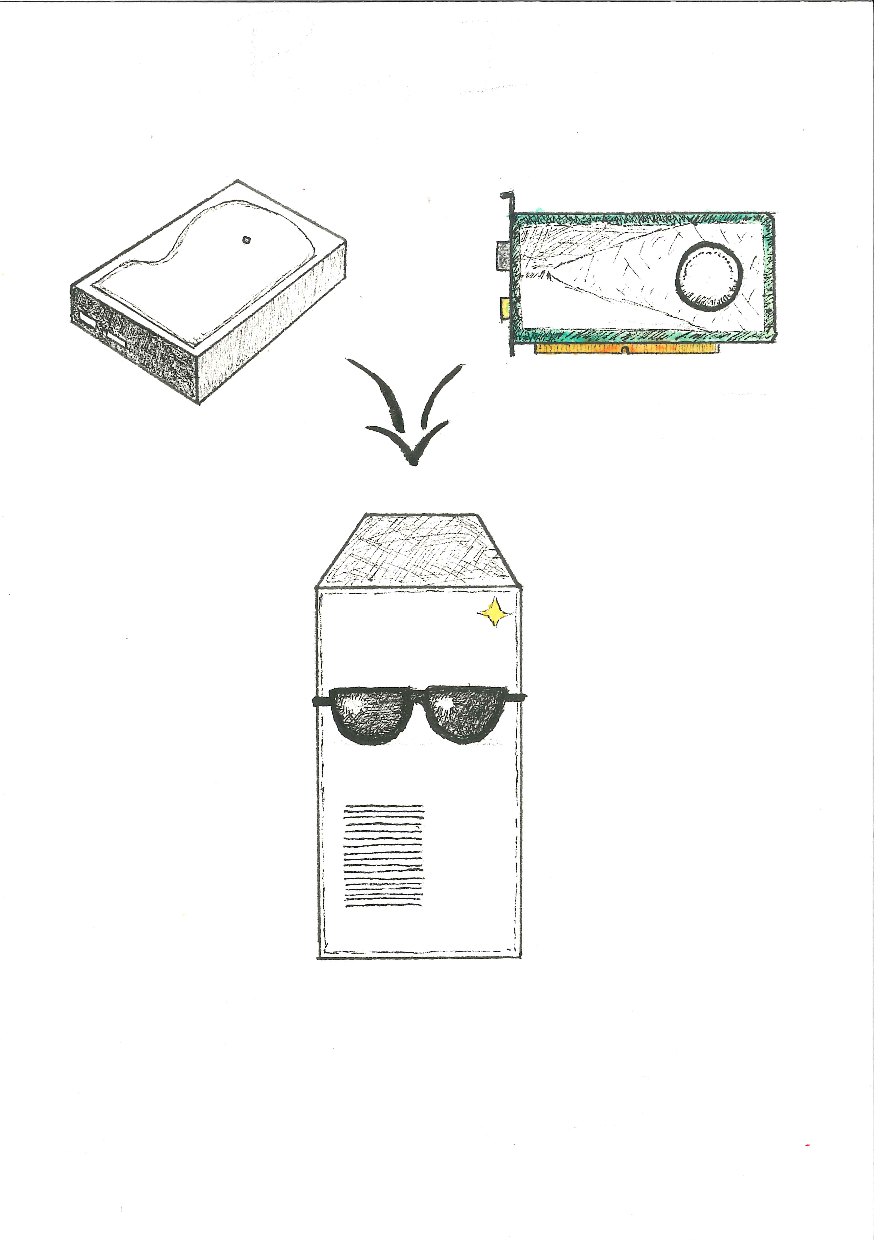
\includegraphics[trim={2mm, 2mm, 2mm, 2mm}, width=0.995\pagewidth]{scans/pg_0007.pdf}};
    
   
    \begin{scope}[x={(image.south east)},y={(image.north west)}]
        \if\helplines1
        	\draw[help lines,xstep=.1,ystep=.1] (0,0) grid (1,1);
        \fi
        \node(title) at (0.5, 0.9) {\Huge {\color{Maroon}I} - ProQ3D};
        \node[align=justify, anchor= west, text width=0.27\pagewidth](en) at (0.04, 0.4) {\english{ProQ3 is a program that tries to predict how good a protein model is.
        		In this paper, we combined the old data with a modern deep learning algorithm in a computer equipped with a GPU.
        		
        		\doindent The result, a “deep” version of ProQ3: ProQ3D.}};
        		
        \node[align=justify, anchor= west, text width=0.28\pagewidth](es) at (0.65, 0.4) {\spanish{ProQ3 es un programa que intenta predecir cómo de preciso es un modelo de una proteína.
        En este artículo, combinamos los datos antiguos con un algoritmo más moderno basado en aprendizaje profundo en un ordenador equipado con una tarjeta gráfica.
        
        \doindent El resultado, una versión <<profunda>> (\emph{\textcolor{Maroon}{“deep”}} en inglés) de ProQ3: ProQ3D.}};
    \end{scope}

\end{tikzpicture}
\end{center}